\documentclass[10pt]{beamer}
\usetheme{metropolis}
\usepackage{booktabs}
\usepackage{tabularx}
\usepackage{calc}
\usepackage{tikz}
\usetikzlibrary{shapes.geometric, arrows, positioning, decorations.pathreplacing, patterns}

% Setup for faculty images
\newlength{\imageheight}
\setlength{\imageheight}{3.5cm}

% Define CSUF brand colors
\definecolor{titanblue}{HTML}{00244E}
\definecolor{mediumblue}{HTML}{0F3F8C}
\definecolor{skyblue}{HTML}{EBFBFF}
\definecolor{titanorange}{HTML}{FF7900}
\definecolor{titangray}{HTML}{F5F5F5}
\definecolor{titantext}{HTML}{222222}

% Customize metropolis theme colors
\setbeamercolor{normal text}{fg=titantext, bg=white}
\setbeamercolor{alerted text}{fg=titanorange}
\setbeamercolor{example text}{fg=mediumblue}

% Title page colors
\setbeamercolor{title}{fg=titanblue, bg=white}
\setbeamercolor{subtitle}{fg=mediumblue, bg=white}
\setbeamercolor{institute}{fg=titanorange, bg=white}
\setbeamercolor{date}{fg=titanblue, bg=white}

% Frame title colors
\setbeamercolor{frametitle}{fg=white, bg=titanblue}
\setbeamercolor{framesubtitle}{fg=mediumblue, bg=white}

% Block environment colors
\setbeamercolor{block title}{fg=white, bg=titanblue}
\setbeamercolor{block body}{fg=titantext, bg=skyblue!10}

% Item colors
\setbeamercolor{itemize item}{fg=titanorange}
\setbeamercolor{itemize subitem}{fg=mediumblue}
\setbeamercolor{itemize subsubitem}{fg=titanblue}

% Footer and header colors
\setbeamercolor{footer}{fg=titantext}
\setbeamercolor{header}{fg=titanblue}

% Customize fonts
\setbeamerfont{title}{size=\Large, series=\bfseries}
\setbeamerfont{frametitle}{size=\large, series=\bfseries}

% Simple title page template
\defbeamertemplate*{title page}{customized}[1][]
{
\vspace{1cm}
 {\usebeamerfont{title}\usebeamercolor[fg]{title}\inserttitle\par}
\vspace{0.5cm}
 {\usebeamerfont{subtitle}\usebeamercolor[fg]{subtitle}\insertsubtitle\par}
\vspace{0.5cm}
 {\usebeamerfont{date}\usebeamercolor[fg]{date}\insertdate\par}
\vfill
 {\insertinstitute\par}
}

% Add progress bar
\makeatletter
\setbeamertemplate{headline}{%
\begin{beamercolorbox}[wd=\paperwidth,ht=0.4cm,dp=0cm]{titanblue}%
\begin{tikzpicture}
\fill[titanorange] (0,0) rectangle (\the\paperwidth*\insertframenumber/\inserttotalframenumber,0.4cm);
\end{tikzpicture}%
\end{beamercolorbox}%
}
\makeatother

\begin{document}

\title{Understanding Politics and Public Policy}
\subtitle{Foundations and Core Concepts\\POSC 315: Introduction to Public Policy\\Lecture 8-2\\Decision Making (Part 2 of 3)}
\author{Dr. David P. Adams}
\date{Summer 2025}
\institute{California State University, Fullerton}

\maketitle

\begin{frame}{Where We Are}
\begin{center}
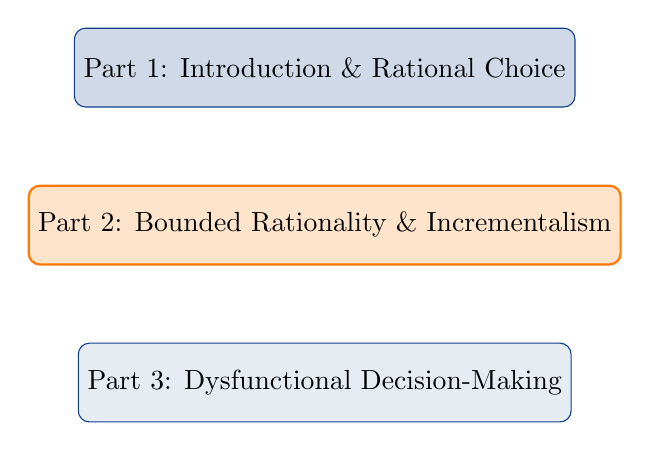
\begin{tikzpicture}[node distance=2cm]
% Define styles
\tikzstyle{completed} = [rectangle, rounded corners, minimum width=3cm, minimum height=1cm, text centered, draw=mediumblue, fill=mediumblue!20]
\tikzstyle{current} = [rectangle, rounded corners, minimum width=3cm, minimum height=1cm, text centered, draw=titanorange, fill=titanorange!20, thick]
\tikzstyle{future} = [rectangle, rounded corners, minimum width=3cm, minimum height=1cm, text centered, draw=mediumblue, fill=mediumblue!10]

% Nodes
\node (part1) [completed] {Part 1: Introduction \& Rational Choice};
\node (part2) [current, below of=part1] {Part 2: Bounded Rationality \& Incrementalism};
\node (part3) [future, below of=part2] {Part 3: Dysfunctional Decision-Making};

\end{tikzpicture}
\end{center}
\end{frame}

\begin{frame}{Recap: Rational Choice Theory}
\begin{center}
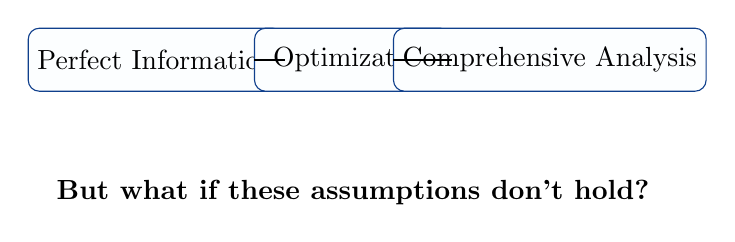
\begin{tikzpicture}[node distance=1.5cm]
\tikzstyle{element} = [rectangle, rounded corners, minimum width=2.5cm, minimum height=0.8cm, text centered, draw=mediumblue, fill=skyblue!15]

\node (perfect) [element] {Perfect Information};
\node (optimize) [element, right of=perfect, xshift=1cm] {Optimization};
\node (comprehensive) [element, right of=optimize, xshift=1cm] {Comprehensive Analysis};

\draw[-, thick] (perfect) -- (optimize);
\draw[-, thick] (optimize) -- (comprehensive);

\node[below=1cm of optimize] {\textbf{But what if these assumptions don't hold?}};

\end{tikzpicture}
\end{center}
\end{frame}

\begin{frame}{Bounded Rationality}
\begin{center}
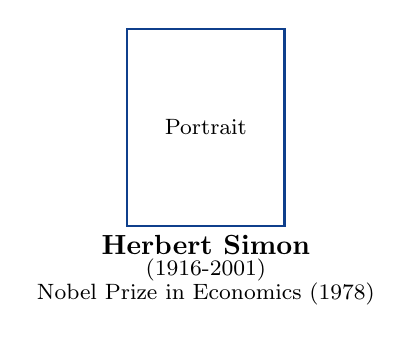
\begin{tikzpicture}
% Portrait placeholder
\draw[thick, mediumblue] (0,0) rectangle (2,2.5);
\node at (1,1.25) {\footnotesize Portrait};
\node[below] at (1,0) {\textbf{Herbert Simon}};
\node[below] at (1,-0.3) {\footnotesize (1916-2001)};
\node[below] at (1,-0.6) {\footnotesize Nobel Prize in Economics (1978)};
\end{tikzpicture}
\end{center}

\begin{block}{Key Quote}
``The capacity of the human mind for formulating and solving complex problems is very small compared with the size of the problems whose solution is required for objectively rational behavior in the real world.''
\end{block}

\begin{frame}{Core Concepts in Bounded Rationality}
\begin{columns}
\begin{column}{0.5\textwidth}
\begin{block}{Intertwined Elements}
\begin{itemize}
\item Goals and tools are considered together
\item Means and ends are not separate
\item Values and facts are interconnected
\end{itemize}
\end{block}
\end{column}
\begin{column}{0.5\textwidth}
\begin{block}{Definition of ``Good'' Policy}
A ``good'' policy is one where \textcolor{titanorange}{\textbf{consensus can be reached}} among stakeholders.
\end{block}
\end{column}
\end{columns}
\end{frame}

\begin{frame}{The ``Administrative Man''}
Bounded rationality recognizes that human rationality is limited:

\vspace{0.5cm}
\begin{center}
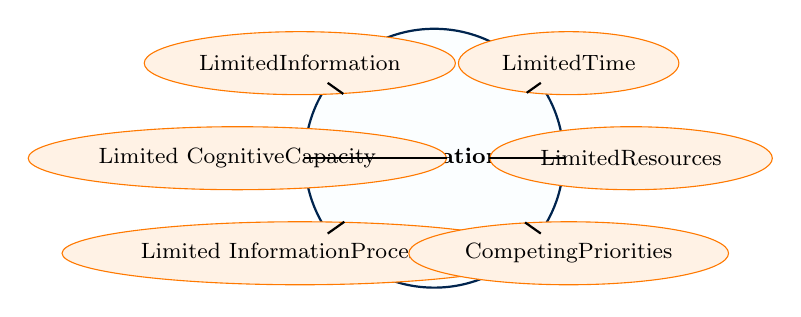
\begin{tikzpicture}[node distance=1cm]
\tikzstyle{constraint} = [ellipse, minimum width=2.8cm, minimum height=0.8cm, text centered, draw=titanorange, fill=titanorange!10]

\node (center) [circle, minimum size=1.5cm, draw=titanblue, fill=skyblue!20, thick] {\footnotesize \textbf{Bounded\\Rationality}};

\node (info) [constraint, above left of=center, xshift=-1cm, yshift=0.5cm] {\footnotesize Limited\\Information};
\node (time) [constraint, above right of=center, xshift=1cm, yshift=0.5cm] {\footnotesize Limited\\Time};
\node (cognitive) [constraint, left of=center, xshift=-1.5cm] {\footnotesize Limited Cognitive\\Capacity};
\node (resources) [constraint, right of=center, xshift=1.5cm] {\footnotesize Limited\\Resources};
\node (processing) [constraint, below left of=center, xshift=-1cm, yshift=-0.5cm] {\footnotesize Limited Information\\Processing};
\node (priorities) [constraint, below right of=center, xshift=1cm, yshift=-0.5cm] {\footnotesize Competing\\Priorities};

% Draw arrows
\foreach \node in {info, time, cognitive, resources, processing, priorities} {
    \draw[-, thick] (\node) -- (center);
}

\end{tikzpicture}
\end{center}
\end{frame}

\begin{frame}{Satisficing in Bounded Rationality}
\begin{center}
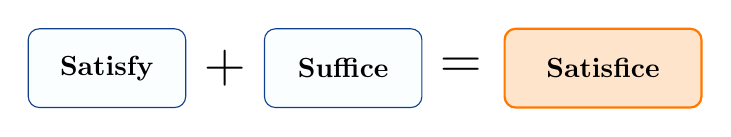
\begin{tikzpicture}[node distance=2cm]
% Create equation-like layout
\node (satisfy) [rectangle, rounded corners, minimum width=2cm, minimum height=1cm, text centered, draw=mediumblue, fill=skyblue!20] {\textbf{Satisfy}};
\node (plus) [right of=satisfy, xshift=-0.5cm] {\huge +};
\node (suffice) [rectangle, rounded corners, minimum width=2cm, minimum height=1cm, text centered, draw=mediumblue, fill=skyblue!20, right of=plus, xshift=-0.5cm] {\textbf{Suffice}};
\node (equals) [right of=suffice, xshift=-0.5cm] {\huge =};
\node (satisfice) [rectangle, rounded corners, minimum width=2.5cm, minimum height=1cm, text centered, draw=titanorange, fill=titanorange!20, thick, right of=equals, xshift=-0.2cm] {\textbf{Satisfice}};

\end{tikzpicture}
\end{center}

\vspace{1cm}
\begin{block}{Key Principles}
\begin{itemize}
\item Administrative actors choose the first option that meets \textcolor{titanorange}{\textbf{minimum criteria}}
\item Makes the most rational decision with available information
\item Achieves satisfactory (not maximum) social gain
\item Recognizes that further search for solutions has costs
\end{itemize}
\end{block}
\end{frame}

\begin{frame}{Rational Choice vs. Bounded Rationality}
\begin{center}
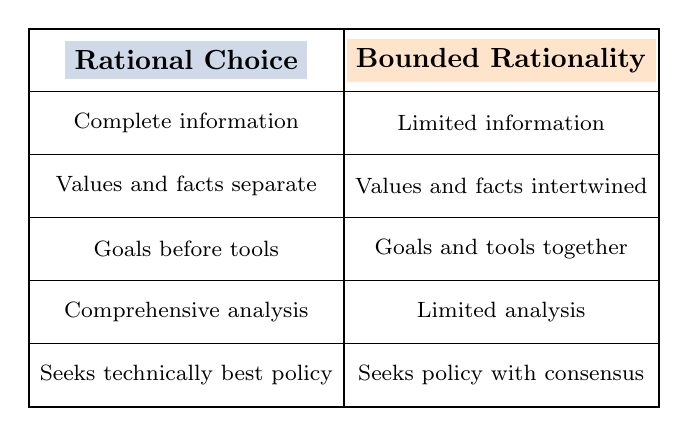
\begin{tikzpicture}[scale=0.8]
% Create comparison table
\draw[thick] (0,0) rectangle (10,6);

% Headers
\node[fill=mediumblue!20] at (2.5,5.5) {\textbf{Rational Choice}};
\node[fill=titanorange!20] at (7.5,5.5) {\textbf{Bounded Rationality}};

% Vertical divider
\draw[thick] (5,0) -- (5,6);

% Row dividers
\foreach \y in {1,2,3,4,5} {
    \draw (0,\y) -- (10,\y);
}

% Left column content
\node[align=center] at (2.5,4.5) {\footnotesize Complete information};
\node[align=center] at (2.5,3.5) {\footnotesize Values and facts separate};
\node[align=center] at (2.5,2.5) {\footnotesize Goals before tools};
\node[align=center] at (2.5,1.5) {\footnotesize Comprehensive analysis};
\node[align=center] at (2.5,0.5) {\footnotesize Seeks technically best policy};

% Right column content
\node[align=center] at (7.5,4.5) {\footnotesize Limited information};
\node[align=center] at (7.5,3.5) {\footnotesize Values and facts intertwined};
\node[align=center] at (7.5,2.5) {\footnotesize Goals and tools together};
\node[align=center] at (7.5,1.5) {\footnotesize Limited analysis};
\node[align=center] at (7.5,0.5) {\footnotesize Seeks policy with consensus};

\end{tikzpicture}
\end{center}
\end{frame}

\begin{frame}{Bounded Rationality: Example}
\begin{block}{Case: City Homelessness Response}
\end{block}

\begin{columns}
\begin{column}{0.5\textwidth}
\textbf{Decision Context}
\begin{itemize}
\item Rising homeless population
\item Mayor facing re-election in 6 months
\item Limited city budget
\item Incomplete data on homeless demographics
\item Multiple stakeholders with competing interests
\end{itemize}
\end{column}
\begin{column}{0.5\textwidth}
\textbf{Satisficing Approach}
\begin{itemize}
\item Review 3-4 policy options (not all possible alternatives)
\item Set minimum criteria: implementable within 4 months, cost under \$2M, address immediate shelter needs
\item Select first option that meets all criteria
\item Choose temporary shelter expansion despite knowing it's not the optimal solution
\end{itemize}
\end{column}
\end{columns}
\end{frame}

\begin{frame}{Incrementalism}
\begin{center}

\begin{tikzpicture}
% Portrait placeholder
\draw[thick, mediumblue] (0,0) rectangle (2,2.5);
\node at (1,1.25) {\footnotesize Portrait};
\node[below] at (1,0) {\textbf{Charles Lindblom}};
\node[below] at (1,-0.3) {\footnotesize (1917-2018)};
\node[below] at (1,-0.6) {\footnotesize ``The Science of Muddling Through'' (1959)};
\end{tikzpicture}
\end{center}

\vspace{0.5cm}
\begin{block}{Foundation}
Builds on Herbert Simon's work on bounded rationality
\begin{itemize}
\item Recognizes limited information processing capacity
\item Focuses on making small, manageable changes
\item Reduces risk through incremental adjustments
\end{itemize}
\end{block}
\end{frame}

\begin{frame}{Successive Limited Comparisons}
\begin{center}
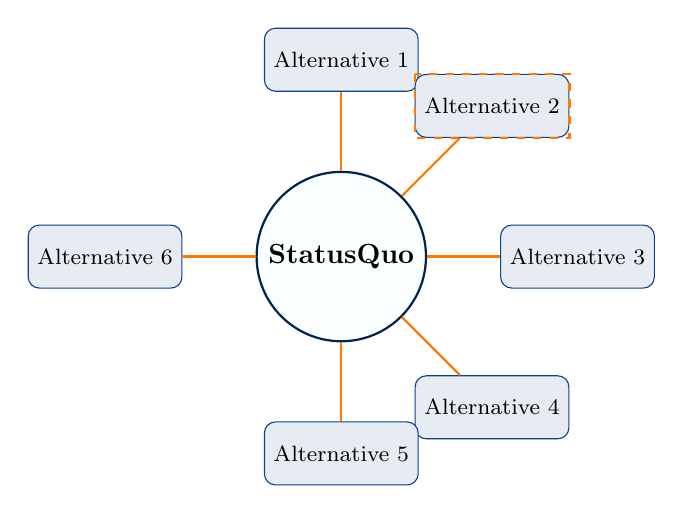
\begin{tikzpicture}[node distance=2cm]
\tikzstyle{statusquo} = [circle, minimum size=2cm, text centered, draw=titanblue, fill=skyblue!20, thick]
\tikzstyle{alternative} = [rectangle, rounded corners, minimum width=1.8cm, minimum height=0.8cm, text centered, draw=mediumblue, fill=mediumblue!10]

% Central status quo
\node (sq) [statusquo] {\textbf{Status\\Quo}};

% Alternatives around it
\node (alt1) [alternative, above of=sq, yshift=0.5cm] {\footnotesize Alternative 1};
\node (alt2) [alternative, above right of=sq, xshift=0.5cm, yshift=0.5cm] {\footnotesize Alternative 2};
\node (alt3) [alternative, right of=sq, xshift=1cm] {\footnotesize Alternative 3};
\node (alt4) [alternative, below right of=sq, xshift=0.5cm, yshift=-0.5cm] {\footnotesize Alternative 4};
\node (alt5) [alternative, below of=sq, yshift=-0.5cm] {\footnotesize Alternative 5};
\node (alt6) [alternative, left of=sq, xshift=-1cm] {\footnotesize Alternative 6};

% Arrows showing small distances
\foreach \alt in {alt1, alt2, alt3, alt4, alt5, alt6} {
    \draw[-, thick, titanorange] (sq) -- (\alt);
}

% Highlight chosen alternative
\draw[titanorange, thick, dashed] (alt2.north west) rectangle (alt2.south east);

\end{tikzpicture}
\end{center}

\vspace{0.5cm}
\begin{itemize}
\item Compare alternatives to the \textcolor{titanorange}{\textbf{status quo}}
\item Choose the alternative that is the \textcolor{titanorange}{\textbf{least different}} from current policy
\end{itemize}
\end{frame}

\begin{frame}{Benefits of Incrementalism}
\begin{columns}
\begin{column}{0.5\textwidth}
\begin{block}{Simplifies Decision-Making}
\begin{itemize}
\item Reduces alternatives to consider
\item Focuses on marginal changes
\item Allows reliance on feedback
\end{itemize}
\end{block}
\end{column}
\begin{column}{0.5\textwidth}
\begin{block}{Manages Risk}
\begin{itemize}
\item Makes process serial and remedial
\item Avoids large, irreversible errors
\item Enables course correction
\end{itemize}
\end{block}
\end{column}
\end{columns}

\vspace{1cm}
\begin{center}
\begin{tikzpicture}[node distance=1.5cm]
\tikzstyle{step} = [rectangle, rounded corners, minimum width=2cm, minimum height=0.8cm, text centered, draw=mediumblue, fill=skyblue!15]

\node (step1) [step] {Small\\Change};
\node (step2) [step, right of=step1] {Assess\\Results};
\node (step3) [step, right of=step2] {Adjust\\Course};
\node (step4) [step, right of=step3] {Next Small\\Change};

\draw[-, thick] (step1) -- (step2);
\draw[-, thick] (step2) -- (step3);
\draw[-, thick] (step3) -- (step4);
\draw[-, thick] (step4) to [bend right=45] (step1);

\end{tikzpicture}
\end{center}
\end{frame}

\begin{frame}{Limitations of Incrementalism}
\begin{block}{Not Always Appropriate}
\begin{itemize}
\item Some problems are too complex for incremental solutions
\item Some problems are too urgent to address incrementally
\item Some problems require fundamental, not incremental, change
\end{itemize}
\end{block}

\vspace{0.5cm}
\textbf{When ``Muddling Through'' Won't Work}

Some decisions require huge leaps:
\begin{itemize}
\item Moonshots \& major technological initiatives
\item Responses to wars \& national security threats
\item Managing pandemics \& public health emergencies
\item Addressing economic depressions \& major recessions
\end{itemize}
\end{frame}

\begin{frame}{Incrementalism: Example}
\begin{block}{Case: Environmental Regulation}
\end{block}

\begin{columns}
\begin{column}{0.5\textwidth}
\textbf{Status Quo}
\begin{itemize}
\item Current emissions standard: 30 parts per million
\item Industry has invested in existing compliance technology
\item Environmental groups want 10ppm standard
\item Economic concerns about rapid changes
\end{itemize}
\end{column}
\begin{column}{0.5\textwidth}
\begin{center}
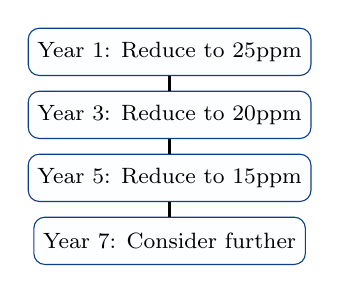
\begin{tikzpicture}[node distance=0.8cm]
\tikzstyle{policystep} = [rectangle, rounded corners, minimum width=3cm, minimum height=0.6cm, text centered, draw=mediumblue, fill=skyblue!15]

\node (year1) [policystep] {\footnotesize Year 1: Reduce to 25ppm};
\node (year3) [policystep, below of=year1] {\footnotesize Year 3: Reduce to 20ppm};
\node (year5) [policystep, below of=year3] {\footnotesize Year 5: Reduce to 15ppm};
\node (year7) [policystep, below of=year5] {\footnotesize Year 7: Consider further};

\draw[-, thick] (year1) -- (year3);
\draw[-, thick] (year3) -- (year5);
\draw[-, thick] (year5) -- (year7);

\end{tikzpicture}
\end{center}

\vspace{0.3cm}
\footnotesize{Each step builds on previous experience and allows for adjustment based on feedback and new information.}
\end{column}
\end{columns}
\end{frame}

\begin{frame}{Three Models Compared}
\begin{center}
\begin{tikzpicture}[node distance=3cm]
\tikzstyle{model} = [rectangle, rounded corners, minimum width=2.5cm, minimum height=2cm, text centered, draw=titanblue, align=center]

\node (rational) [model, fill=mediumblue!10] {\textbf{Rational\\Choice}\\[0.3cm]\footnotesize Complete info\\Optimization\\Comprehensive};
\node (bounded) [model, fill=mediumblue!20, right of=rational] {\textbf{Bounded\\Rationality}\\[0.3cm]\footnotesize Limited info\\Satisficing\\Consensus};
\node (incremental) [model, fill=mediumblue!30, right of=bounded] {\textbf{Incrementalism}\\[0.3cm]\footnotesize Small changes\\Status quo\\Serial process};

% Decision complexity arrow
\draw[very thick, titanorange] ([yshift=-1cm]rational.south) -- ([yshift=-1cm]incremental.south);
\node[below] at ([yshift=-1.3cm]bounded.south) {\footnotesize Increasing practical applicability};

\end{tikzpicture}
\end{center}
\end{frame}

\begin{frame}{When to Use Each Model}
\begin{center}
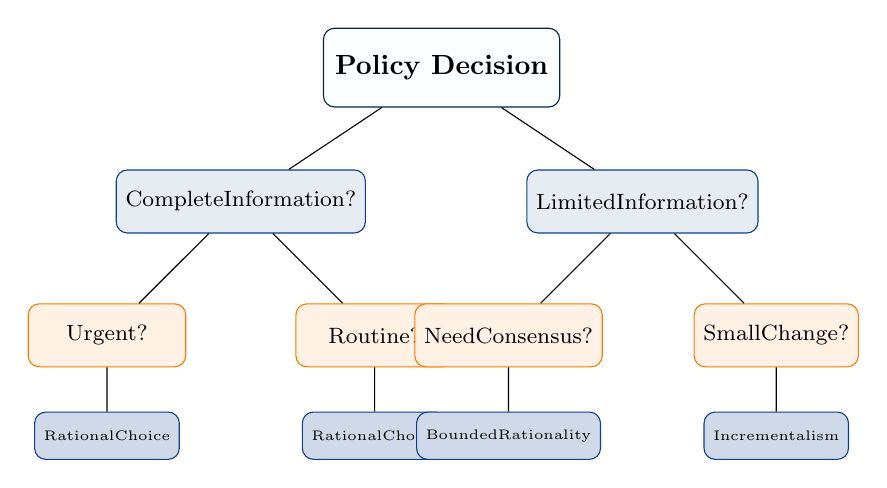
\begin{tikzpicture}[scale=0.85]
% Create decision tree
\node[rectangle, rounded corners, minimum width=3cm, minimum height=1cm, text centered, draw=titanblue, fill=skyblue!20] (start) at (0,0) {\textbf{Policy Decision}};

% First branch - information availability
\node[rectangle, rounded corners, minimum width=2.5cm, minimum height=0.8cm, text centered, draw=mediumblue, fill=mediumblue!10] (complete) at (-3,-2) {\footnotesize Complete\\Information?};
\node[rectangle, rounded corners, minimum width=2.5cm, minimum height=0.8cm, text centered, draw=mediumblue, fill=mediumblue!10] (limited) at (3,-2) {\footnotesize Limited\\Information?};

% Second branch - urgency
\node[rectangle, rounded corners, minimum width=2cm, minimum height=0.8cm, text centered, draw=titanorange, fill=titanorange!10] (urgent) at (-5,-4) {\footnotesize Urgent?};
\node[rectangle, rounded corners, minimum width=2cm, minimum height=0.8cm, text centered, draw=titanorange, fill=titanorange!10] (routine) at (-1,-4) {\footnotesize Routine?};
\node[rectangle, rounded corners, minimum width=2cm, minimum height=0.8cm, text centered, draw=titanorange, fill=titanorange!10] (consensus) at (1,-4) {\footnotesize Need\\Consensus?};
\node[rectangle, rounded corners, minimum width=2cm, minimum height=0.8cm, text centered, draw=titanorange, fill=titanorange!10] (incremental) at (5,-4) {\footnotesize Small\\Change?};

% Final recommendations
\node[rectangle, rounded corners, minimum width=1.8cm, minimum height=0.6cm, text centered, draw=mediumblue, fill=mediumblue!20] (rc1) at (-5,-5.5) {\tiny Rational\\Choice};
\node[rectangle, rounded corners, minimum width=1.8cm, minimum height=0.6cm, text centered, draw=mediumblue, fill=mediumblue!20] (rc2) at (-1,-5.5) {\tiny Rational\\Choice};
\node[rectangle, rounded corners, minimum width=1.8cm, minimum height=0.6cm, text centered, draw=mediumblue, fill=mediumblue!20] (br) at (1,-5.5) {\tiny Bounded\\Rationality};
\node[rectangle, rounded corners, minimum width=1.8cm, minimum height=0.6cm, text centered, draw=mediumblue, fill=mediumblue!20] (inc) at (5,-5.5) {\tiny Incrementalism};

% Draw connections
\draw[-] (start) -- (complete);
\draw[-] (start) -- (limited);
\draw[-] (complete) -- (urgent);
\draw[-] (complete) -- (routine);
\draw[-] (limited) -- (consensus);
\draw[-] (limited) -- (incremental);
\draw[-] (urgent) -- (rc1);
\draw[-] (routine) -- (rc2);
\draw[-] (consensus) -- (br);
\draw[-] (incremental) -- (inc);

\end{tikzpicture}
\end{center}
\end{frame}

\begin{frame}{Key Takeaways: Alternative Models}
\begin{center}
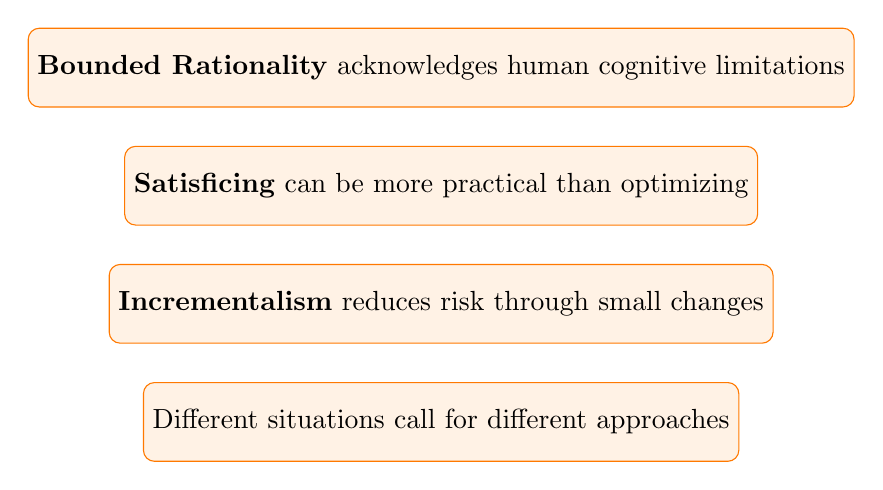
\begin{tikzpicture}[node distance=1.5cm]
\tikzstyle{takeaway} = [rectangle, rounded corners, minimum width=7cm, minimum height=1cm, text centered, draw=titanorange, fill=titanorange!10]

\node (t1) [takeaway] {\textbf{Bounded Rationality} acknowledges human cognitive limitations};
\node (t2) [takeaway, below of=t1] {\textbf{Satisficing} can be more practical than optimizing};
\node (t3) [takeaway, below of=t2] {\textbf{Incrementalism} reduces risk through small changes};
\node (t4) [takeaway, below of=t3] {Different situations call for different approaches};

\end{tikzpicture}
\end{center}
\end{frame}

\begin{frame}{Looking Ahead}
\begin{center}
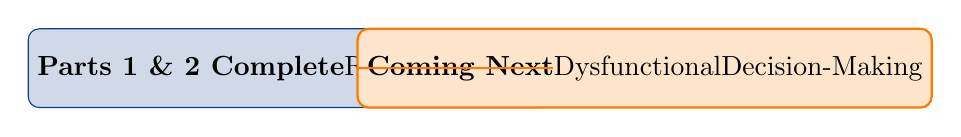
\begin{tikzpicture}[node distance=2cm]
\tikzstyle{progressCompleted} = [rectangle, rounded corners, minimum width=3.5cm, minimum height=1cm, text centered, draw=mediumblue, fill=mediumblue!20]
\tikzstyle{progressNext} = [rectangle, rounded corners, minimum width=3.5cm, minimum height=1cm, text centered, draw=titanorange, fill=titanorange!20, thick]

\node (current) [progressCompleted] {\textbf{Parts 1 \& 2 Complete}\\Rational Models};
\node (part3) [progressNext, right of=current, xshift=2.5cm] {\textbf{Coming Next}\\Dysfunctional\\Decision-Making};

\draw[-, thick, titanorange] (current) -- (part3);

\end{tikzpicture}
\end{center}

\vspace{1cm}
\textbf{Next time we'll explore:}
\begin{itemize}
\item Groupthink and its dangers
\item The Garbage Can Model
\item When decision-making goes wrong
\item Safeguards against dysfunction
\end{itemize}
\end{frame}

\end{document}